\section{Extensions}

\subsection{Evidence} \label{sect:evidence}

In work many studies on the area of multiagent communication models, there exists a ``true state'' of the world that the agents must confer in order to agree upon. Here we will explore the effects of including such a feature. Firstly, we arbitrarily assign one state of the world to be ``true''. Then at each iteration the simulation conducts $K$ Bernoulli trials with probability $\pi$ in order to establish which agents in the population will receive some evidence. Secondly, there is a chance $c$ that the evidence is accurate. This can be thought of as an agent querying an external, inaccurate oracle. Here, the oracle returns an argument of the same form as $\mathbf{A}$ that is incorporated into an agents beliefs as described in~\cref{eq:BU_update_rule}. 

One might expect the introduction of this true state to sway the agents towards the true state of the world when $c > 0.5, \pi > 0$, an observation supported by~\cref{fig:evidence}. In this figure, the true state of the world is rotated on the $2,000^{\textnormal{th}},5,000^{\textnormal{th}},10,000^{\textnormal{th}} $ and $ 20,000^{\textnormal{th}}$ iterations. \cref{fig:evidence_deviation} shows the average J-Divergence between the true state of the world and each agent at each timestep, referred to as the deviation. 


\begin{figure}[H]
 \centering
  \begin{subfigure}[ht]{0.45\textwidth}
    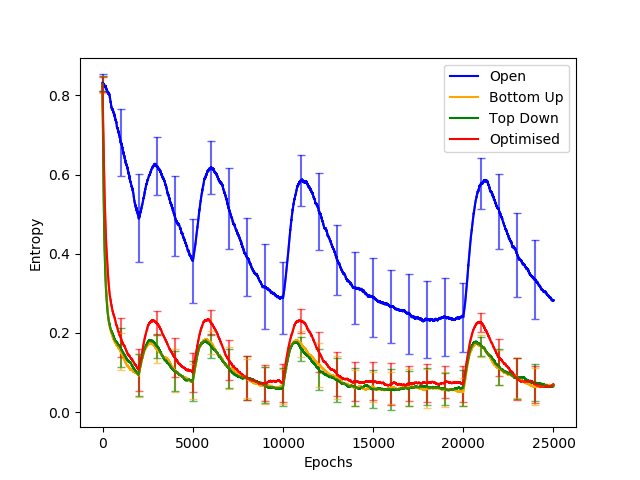
\includegraphics[width=\textwidth]{Images/Figures/Evidence/EntropyGood.png}
    \caption{Entropy}
 \end{subfigure}
 \hfill
 \begin{subfigure}[ht]{0.45\textwidth}
    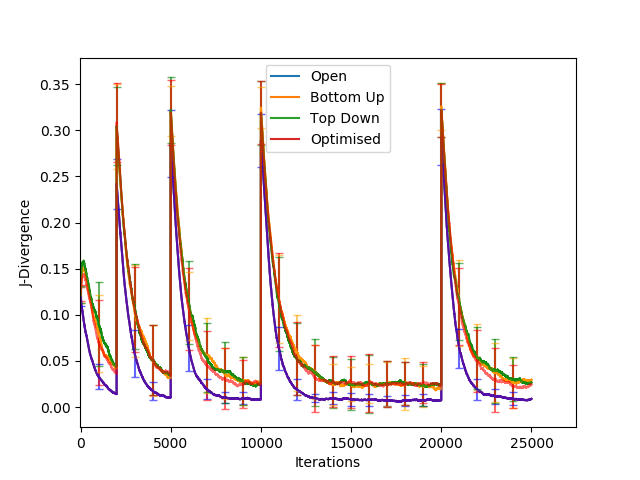
\includegraphics[width=\textwidth]{Images/Figures/Evidence/J-DivGood.png}
    \caption{Deviation} \label{fig:evidence_deviation}
 \end{subfigure}
 \caption{Two plots showing entropy and J-Divergence over $25,000$ iterations for the Open, Bottom Up, Top Down and Optimised models, with simple listeners. At the $2,000^{\textnormal{th}},5,000^{\textnormal{th}},10,000^{\textnormal{th}} $ and $ 20,000^{\textnormal{th}} $, the true state of the world is switched to be $H_{i+1}$, highlighted by the jumps in deviation between the true state and each agent.}\label{fig:evidence}
\end{figure}

It can be seen in this figure that the Open model has higher entropy on average than the other models, as described above, but that they cluster together slightly quicker that the rest. When the true state changes, all the models recover, updating their beliefs toward the true state as they receive more and more evidence in its favour, however, it can be seen that the Open model, on average gets the population closer to the true state. Consider an agent $i$ that is undecided between two states, with a set of beliefs $P_{i} = [0.4, 0.6, 0]$. Now, let the true state be $H_1$, which the majority of the population believes to be the most credible state, including the listener. If agent $i$ is selected to speak as a Bottom Up agent, it will simply assert $H_2$, whereas, if it is speaking as an Open agent, it will assert $[0.4, 0.6, 0]$. It is clear that the absolute nature of the first assertion will cause a larger update in the listener, updating it away from the true state. This process will balance with the rate at which inaccurate evidence is received accounting for the difference between the deviation of the Open and other models.


\subsection{Reconstructive}

One of the assumptions made in the above models is that the agents have perfect information, an attribute that only the Optimised model makes full use of. In this model, the speaker creates the argument that will cause the listener to update their beliefs to be as close as possible to the speaker. To do that, the speaker must inspect the exact nature of the listeners beliefs, which it can do due to its perfect information. However, this is highly unrealistic, as it is rare that any agent will not only be so open and well understood. To weaken this assumption we can attempt to reconstruct the listeners beliefs based on their previous assertions.

Let each agent in the population keep a record of the last $\zeta$ assertions the speaker has made in the set $\mathbf{A}_\zeta$. It is likely that these assertions will reflect an agents set of beliefs in aggregate. Hence, the speaker takes an average of the last $\zeta$ assertions by the listener to approximate their beliefs at the current timestep, renormalising it to be a probability distribution. This approximation takes the form

\begin{equation} \label{eq:reconstructive}
    \hat{P}_{Li} = \frac{\abs{ \{H_i: H_i \in \mathbf{A}_\zeta \} } }{ \sum_j^n \abs{ \{ H_j; H_j \in \mathbf{A}_\zeta \} }   }
\end{equation}

\Cref{fig:reconstructive}


\begin{figure}[H]
 \centering
  \begin{subfigure}[ht]{0.45\textwidth}
    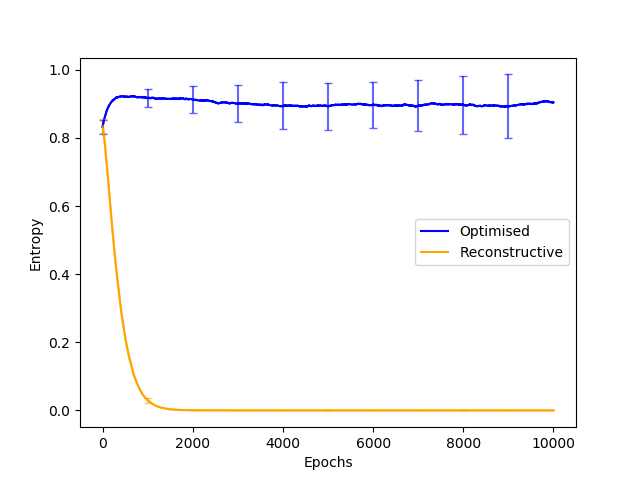
\includegraphics[width=\textwidth]{Images/Figures/Reconstructive/Entropy_reconstruct.png}
    \caption{Entropy}
 \end{subfigure}
 \hfill
 \begin{subfigure}[ht]{0.45\textwidth}
    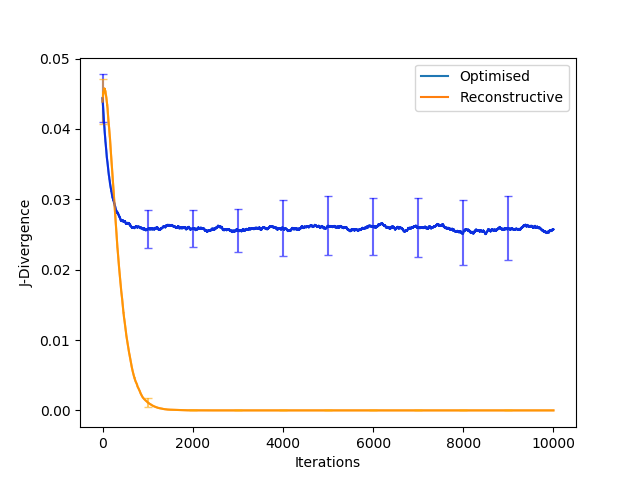
\includegraphics[width=\textwidth]{Images/Figures/Reconstructive/J-Div_reconstruct.png}
    \caption{J-Divergence}
 \end{subfigure}
 \caption{Two plots showing entropy and J-Divergence over time for the Optimised and Reconstructive models, with simple listeners. \textit{Computed using $K = 100, n=3, \alpha = 0.5, \zeta = 10$}}\label{fig:reconstructive}
\end{figure}



\subsection{Population Tests}

In Economics, agents can be assigned a variety of different trading strategies, with the aim of making deals that maximise the agents profit. The earliest mechanisms proposed were rudimentary, such as ZI-U and ZI-C~\cite{Gode1993AllocativeRationality}, with later models incorporated machine learning techniques to improve their performance, such as ZI-P, GDX and AA~\cite{CliffMinimal-IntelligenceEnvironments, GjerstadPriceAuctions, Vytelingum2006TheAuction}. \cite{Vach2015ComparisonAgents} provides an excellent comparison of the dynamics of having a population of agents practising different strategies, pursuing the same goal, inspiring the following analysis. In order to determining the most persuasive argumentation strategy, we must maintain a record of the J-Divergence of an agent before and after it receives an argument from a particular type of agent. This indicates the amount of movement in the population each strategy can claim responsibility for. Furthermore, different concentrations of each strategy should be considered, as, in Vach's work, some strategies perform best when in a minority. 

The following table shows the mean and variance of the J-Divergence, summed for each agent across $5,000$ iterations for a population of $100$ agents mixed to the corresponding concentrations. It also shows the fraction of those $1,000$ runs that was ``won'' by each strategy, the victors shown in bold. 

\begin{table}[H]
\begin{adjustbox}{max width = \textwidth}
\begin{tabular}{ll||cc|cc|cc|cc|cc|cc}
 &  & Open & Bottom Up & Open & Top Down & Open & Optimised & Bottom Up & Top Down & Bottom Up & Optimised & Top Down & Optimised \\ \hline \hline
\multirow{3}{*}{1:5} & Wins & 0 & \textbf{1000} & 0 & \textbf{1000} & 0 & \textbf{1000} & 0 & \textbf{1000} & 0 & \textbf{1000} & 0 & \textbf{1000} \\
 & Mean & 102.62 & 556.77 & 266.24 & 310.25 & 32.71 & 461.35 & 116.48 & 572.93 & 98.44 & 559.44 & 114.65 & 537.71 \\
 & Variance & 1148.21 & 33438.32 & 6921.15 & 9352.62 & 109.91 & 27371.37 & 1392.15 & 31723.34 & 976.91 & 28583.10 & 1172.33 & 25994.92 \\ \hline
\multirow{3}{*}{2:4} & Wins & 0 & \textbf{1000} & 0 & \textbf{1000} & 0 & \textbf{1000} & 0 & \textbf{1000} & 0 & \textbf{1000} & 0 & \textbf{1000} \\
 & Mean & 195.84 & 434.74 & 196.56 & 439.31 & 63.32 & 301.55 & 237.99 & 465.36 & 197.7 & 459.79 & 235.58 & 573.71 \\
 & Variance & 3854.64 & 19181.86 & 3813.80 & 18625.79 & 471.60 & 14043.25 & 5053.55 & 31723.34 & 4233.75 & 19309.38 & 1172.33 & 17252.55 \\ \hline
\multirow{3}{*}{3:3} & Wins & 15 & \textbf{985} & 2 & \textbf{998} & 0 & \textbf{1000} & \textbf{763} & 237 & 0 & \textbf{1000} & 25 & \textbf{975} \\
 & Mean & 259.22 & 298.03 & 268.98 & 313.77 & 91.57 & 191.49 & 340.28 & 328.92 & 300.58 & 357.97 & 345.47 & 377.57 \\
 & Variance & 7659.79 & 10325.40 & 7443.46 & 10013.92 & 1033.30 & 5834.30 & 12284.39 & 11320.51 & 10007.85 & 10921.99 & 11334.45 & 10525.32 \\ \hline
\multirow{3}{*}{4:2} & Wins & \textbf{1000} & 0 & \textbf{1000} & 0 & \textbf{757} & 243 & \textbf{1000} & 0 & \textbf{997} & 3 & \textbf{1000} & 0 \\
 & Mean & 275.46 & 168.0 & 296.03 & 186.38 & 114.61 & 109.65 & 470.81 & 223.92 & 421.71 & 256.17 & 471.36 & 267.90 \\
 & Variance & 10258.49 & 4066.55 & 10228.22 & 4070.70 & 1515.69 & 1834.65 & 20385.43 & 4530.30 & 18896.96 & 4640.16 & 18313.40 & 4027.28 \\ \hline
\multirow{3}{*}{5:1} & Wins & 10 & \textbf{990} & \textbf{1000} & 0 & \textbf{1000} & 0 & \textbf{1000} & 0 & \textbf{1000} & 0 & \textbf{1000} & 0 \\
 & Mean & 261.47 & 300.25 & 242.22 & 76.76 & 125.61 & 50.62 & 571.24 & 109.50 & 541.02 & 139.20 & 585.96 & 143.79 \\
 & Variance & 7698.04 & 10595.29 & 7969.72 & 850.05 & 1640.94 & 386.30 & 32849.13 & 1223.31 & 31937.07 & 1127.97 & 29570.50 & 996.34
\end{tabular}
\end{adjustbox}
\caption{Table to show results of mixing different persuasion strategies together in different concentrations, with simple listeners. The victor of the majority of the $1,000$ games is shown in bold, alongside the mean and variance J-Divergence each strategy is responsible for. }
\end{table}


The results of this experiment are much as one would expect, showing that, in almost all cases, the agent in the majority is responsible for the most movement in the population. However, there are some cases where the strategy is not universally superior, for instance, the Open vs Optimised games with a $4:2$ concentration shows the Optimised solution winning $24.3 \%$ of the time. This shows the limitations of the Open model, as demonstrated in~\cref{sect:evidence}, with its more diluted arguments limiting the potency of the argument. Another remarkable observation is the result of the Open vs Bottom Up game with a $5:1$ concentration. 
\todo{I have no idea why this happened}

It can also be seen that the Optimised model appears to dominate the balanced group tests, only losing $25$ games to the Top Down model. This suggests that its ability to assert anything it must to change the listener's beliefs toward the speaker causes a large amount of movement in the population, at least during the first $5,000$ iterations. 

In these tests, some differences between the Top Down and Bottom Up models can be seen. 